% ============================================================
\chapter{Introduction to Relational Databases}
\label{ch:introduction}
% ============================================================

In 1970, Edgar F.\ Codd, a researcher at IBM, published a paper that would
revolutionize computing: \emph{A Relational Model of Data for Large Shared
Data Banks}. His idea: organize data into \emph{tables} connected by precise
algebraic operations, radically separating how data is physically stored
from how it is logically queried. IBM, in an irony of history, took years to
implement its own researcher's ideas --- it was a group at Berkeley, led by
Michael Stonebraker, that created the first practical relational system.
Today, relational databases store the bulk of the world's information.

% ------------------------------------------------------------
\section{What Is a Database?}
% ------------------------------------------------------------

Let us begin with the most fundamental question.

\begin{definition}[Database]
A \emph{database} is an organized collection of structured data, stored
persistently and accessible by multiple users and applications in a
controlled manner.
\end{definition}

Unlike a simple flat file (CSV, text), a database provides:
\begin{itemize}
    \item \textbf{Persistence} --- data survives program termination.
    \item \textbf{Sharing} --- multiple users access data concurrently.
    \item \textbf{Integrity} --- constraints ensure data consistency.
    \item \textbf{Security} --- access control mechanisms protect data.
    \item \textbf{Efficient querying} --- a declarative language (SQL) lets users
          ask complex questions without specifying ``how.''
\end{itemize}

\begin{example}
Consider a university management system. Without a database, we might store
students in a CSV file:
\begin{verbatim}
1,Brown,Alice,2004-03-15,CS
2,Davis,Bob,2003-11-22,CS
\end{verbatim}
Problems: no type checking, no foreign keys, no safe concurrent access,
no efficient complex queries.
\end{example}

\section{A Brief History}

\begin{enumerate}
    \item \textbf{1960s} --- File systems, hierarchical models (IBM's IMS) and
          network models (CODASYL). Data organized as trees or graphs with
          explicit navigation.
    \item \textbf{1970} --- Edgar F.~Codd publishes \emph{``A Relational Model of Data
          for Large Shared Data Banks,''} laying the foundations of the relational
          model. Data is organized in \emph{tables} (relations) manipulated by
          set-based operators.
    \item \textbf{1970s--80s} --- Development of System R (IBM) and Ingres (Berkeley);
          birth of SQL (originally SEQUEL).
    \item \textbf{1980s--90s} --- Commercialization: Oracle, DB2, SQL Server,
          PostgreSQL. SQL standardization (SQL-86, SQL-92, SQL:1999).
    \item \textbf{2000s} --- Object-oriented databases, XML, data warehouses.
    \item \textbf{2010s+} --- NoSQL explosion (MongoDB, Cassandra, Neo4j),
          NewSQL, in-memory databases, data lakes.
\end{enumerate}

\begin{remark}
Despite the rise of NoSQL, the relational model remains the most widely used
in industry. SQL skills are among the most sought-after on the IT job market.
\end{remark}

\section{Database Management Systems (DBMS)}

\begin{definition}[DBMS]
A \emph{Database Management System} (DBMS) is software that enables creating,
managing, and querying databases. It ensures independence between application
programs and the physical representation of data.
\end{definition}

A DBMS provides the following functions (Codd's rules):
\begin{itemize}
    \item \textbf{Data Definition} (DDL) --- creating tables, constraints, indexes.
    \item \textbf{Data Manipulation} (DML) --- inserting, updating, deleting, querying.
    \item \textbf{Data Control} (DCL) --- access rights, roles.
    \item \textbf{Transaction Control} (TCL) --- \texttt{BEGIN}, \texttt{COMMIT}, \texttt{ROLLBACK}.
\end{itemize}

\subsection{Three-Level Architecture (ANSI/SPARC)}

\begin{definition}[ANSI/SPARC Architecture]
The ANSI/SPARC architecture (1975) defines three levels of abstraction:
\begin{enumerate}
    \item \textbf{External level} (user views) --- each user or application
          sees an adapted subset of the data.
    \item \textbf{Conceptual level} (logical schema) --- complete description
          of the data structure, independent of physical storage.
    \item \textbf{Internal level} (physical schema) --- on-disk organization:
          files, indexes, partitions.
\end{enumerate}
\end{definition}

\begin{center}
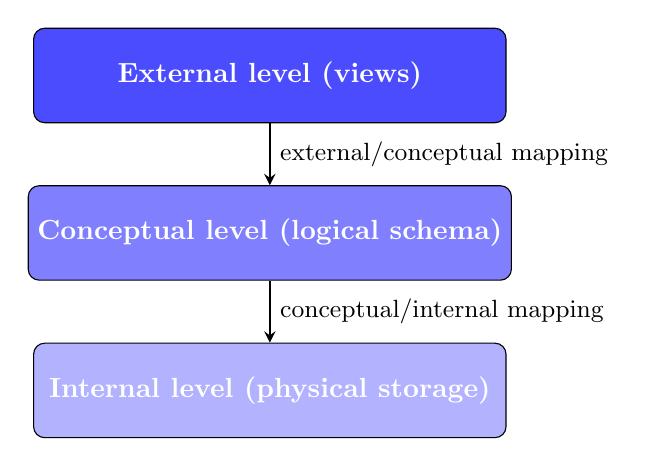
\begin{tikzpicture}[
    niveau/.style={draw, rounded corners, minimum width=6cm, minimum height=1.2cm,
                   font=\bfseries, text=white},
    fleche/.style={->, thick, >=stealth}
]
    \node[niveau, fill=blue!70] (ext) at (0,4) {External level (views)};
    \node[niveau, fill=blue!50] (con) at (0,2) {Conceptual level (logical schema)};
    \node[niveau, fill=blue!30] (int) at (0,0) {Internal level (physical storage)};

    \draw[fleche] (ext) -- (con) node[midway, right, font=\small] {external/conceptual mapping};
    \draw[fleche] (con) -- (int) node[midway, right, font=\small] {conceptual/internal mapping};
\end{tikzpicture}
\end{center}

\begin{theorem}[Data Independence]
The three-level architecture guarantees two forms of independence:
\begin{itemize}
    \item \textbf{Logical independence}: the conceptual schema can be modified
          without affecting external views.
    \item \textbf{Physical independence}: the physical organization (adding
          indexes, changing file format) can be modified without affecting
          the conceptual schema.
\end{itemize}
\end{theorem}

\section{The Relational Model}

\begin{definition}[Relation]
Let $D_1, D_2, \ldots, D_n$ be domains (sets of possible values).
A \emph{relation} $R$ with schema $R(A_1:D_1, A_2:D_2, \ldots, A_n:D_n)$
is a finite subset of the Cartesian product $D_1 \times D_2 \times \cdots \times D_n$.
Each element of $R$ is called a \emph{tuple}.
\end{definition}

\begin{keyformulas}[title=\textbf{Relational vs.\ Tabular Terminology}]
\begin{center}
\begin{tabular}{lll}
\toprule
\textbf{Relational Model} & \textbf{Table} & \textbf{SQL} \\
\midrule
Relation & Table & \texttt{TABLE} \\
Attribute & Column & \texttt{COLUMN} \\
Tuple & Row & \texttt{ROW} \\
Domain & Data type & \texttt{INTEGER}, \texttt{TEXT}, \ldots \\
Degree & Number of columns & --- \\
Cardinality & Number of rows & \texttt{COUNT(*)} \\
\bottomrule
\end{tabular}
\end{center}
\end{keyformulas}

\begin{definition}[Candidate Key and Primary Key]
Let $R$ be a relation with schema $R(A_1, \ldots, A_n)$.
\begin{itemize}
    \item A \emph{superkey} of $R$ is a subset $K \subseteq \{A_1, \ldots, A_n\}$
          such that for any two distinct tuples $t_1, t_2 \in R$, we have $t_1[K] \neq t_2[K]$.
    \item A \emph{candidate key} is a minimal superkey (no proper subset is
          itself a superkey).
    \item The \emph{primary key} is the candidate key chosen by the designer to
          uniquely identify each tuple.
\end{itemize}
\end{definition}

\begin{example}
In the \texttt{Students} table:
\begin{itemize}
    \item $\{$\texttt{student\_id}$\}$ is a candidate key (and the chosen primary key).
    \item $\{$\texttt{last\_name}, \texttt{first\_name}, \texttt{birth\_date}$\}$ could
          be a candidate key if we assume uniqueness of this combination.
    \item $\{$\texttt{student\_id}, \texttt{last\_name}$\}$ is a superkey but not a
          candidate key (not minimal).
\end{itemize}
\end{example}

\begin{definition}[Foreign Key]
Given two relations $R$ and $S$, a set of attributes $FK$ of $R$ is a
\emph{foreign key} referencing $S$ if, for every tuple $t \in R$,
$t[FK]$ is either \texttt{NULL} or equal to $s[PK]$ for some tuple $s \in S$,
where $PK$ is the primary key of $S$.
\end{definition}

\section{DBMS Languages}

\subsection{DDL --- Data Definition Language}

\begin{codeblock}[title=\textbf{Creating a Table with Constraints}]
\begin{minted}{sql}
CREATE TABLE Students (
    student_id   INTEGER PRIMARY KEY,
    last_name    TEXT NOT NULL,
    first_name   TEXT NOT NULL,
    birth_date   DATE,
    major        TEXT CHECK (major IN ('CS', 'Math', 'Physics')),
    UNIQUE (last_name, first_name, birth_date)
);
\end{minted}
\end{codeblock}

\subsection{DML --- Data Manipulation Language}

\begin{codeblock}[title=\textbf{Basic CRUD Operations}]
\begin{minted}{sql}
-- Create (insert)
INSERT INTO Students (student_id, last_name, first_name, major)
VALUES (6, 'Garcia', 'Lucy', 'CS');

-- Read (query)
SELECT last_name, first_name FROM Students WHERE major = 'CS';

-- Update
UPDATE Students SET major = 'Math' WHERE student_id = 6;

-- Delete
DELETE FROM Students WHERE student_id = 6;
\end{minted}
\end{codeblock}

\subsection{DCL --- Data Control Language}

\begin{codeblock}[title=\textbf{Access Control (PostgreSQL)}]
\begin{minted}{sql}
-- Grant read access
GRANT SELECT ON Students TO web_user;

-- Grant all privileges
GRANT ALL PRIVILEGES ON Courses TO admin_user;

-- Revoke a privilege
REVOKE DELETE ON Students FROM web_user;
\end{minted}
\end{codeblock}

\section{Major Relational DBMS}

\begin{center}
\begin{tabular}{llll}
\toprule
\textbf{DBMS} & \textbf{License} & \textbf{Typical Use} & \textbf{Highlight} \\
\midrule
PostgreSQL & Open source & Enterprise, web & Highly SQL-compliant \\
MySQL/MariaDB & Open source & Web (LAMP) & Very widespread \\
SQLite & Public domain & Embedded, mobile & Serverless \\
Oracle DB & Commercial & Large enterprise & High performance \\
SQL Server & Commercial & Enterprise (.NET) & Microsoft integration \\
\bottomrule
\end{tabular}
\end{center}

\section{Getting Started with SQLite and Python}

SQLite is built into Python via the \texttt{sqlite3} module:

\begin{codeblock}[title=\textbf{Connecting and Creating Tables with Python}]
\begin{minted}{python}
import sqlite3

# Connect (creates the file if it does not exist)
conn = sqlite3.connect('university.db')
cur = conn.cursor()

# Create the table
cur.execute('''
    CREATE TABLE IF NOT EXISTS Students (
        student_id   INTEGER PRIMARY KEY,
        last_name    TEXT NOT NULL,
        first_name   TEXT NOT NULL,
        birth_date   DATE,
        major        TEXT
    )
''')

# Insert data
cur.execute("INSERT INTO Students VALUES (1, 'Brown', 'Alice', '2004-03-15', 'CS')")
cur.execute("INSERT INTO Students VALUES (2, 'Davis', 'Bob', '2003-11-22', 'CS')")

conn.commit()

# Query
cur.execute("SELECT * FROM Students")
for row in cur.fetchall():
    print(row)

conn.close()
\end{minted}
\end{codeblock}

\begin{codeoutput}
\begin{verbatim}
(1, 'Brown', 'Alice', '2004-03-15', 'CS')
(2, 'Davis', 'Bob', '2003-11-22', 'CS')
\end{verbatim}
\end{codeoutput}

\begin{bestpractice}[title=\textbf{Use Parameterized Queries}]
Never build SQL queries by string concatenation: this exposes you to
\emph{SQL injection attacks}. Use parameter placeholders (\texttt{?}):
\begin{minted}{python}
# GOOD: parameterized query
cur.execute("SELECT * FROM Students WHERE major = ?", ('CS',))

# BAD: string concatenation (SQL injection possible!)
# cur.execute("SELECT * FROM Students WHERE major = '" + major + "'")
\end{minted}
\end{bestpractice}

\section{SQL Data Types}

\begin{keyformulas}[title=\textbf{Common SQL Data Types}]
\begin{center}
\begin{tabular}{lll}
\toprule
\textbf{Category} & \textbf{SQL Type} & \textbf{Description} \\
\midrule
Integer & \texttt{INTEGER}, \texttt{SMALLINT}, \texttt{BIGINT} & Whole numbers \\
Real & \texttt{REAL}, \texttt{FLOAT}, \texttt{DOUBLE} & Floating-point numbers \\
Decimal & \texttt{NUMERIC(p,s)}, \texttt{DECIMAL} & Exact precision \\
Text & \texttt{TEXT}, \texttt{VARCHAR(n)}, \texttt{CHAR(n)} & Character strings \\
Date/Time & \texttt{DATE}, \texttt{TIME}, \texttt{TIMESTAMP} & Temporal data \\
Boolean & \texttt{BOOLEAN} & True/false \\
Binary & \texttt{BLOB} & Binary data \\
\bottomrule
\end{tabular}
\end{center}
\end{keyformulas}

\begin{warning}[title=\textbf{NULL Is Not Zero}]
The value \texttt{NULL} represents the absence of a value. It differs from
$0$, the empty string \texttt{''}, or \texttt{FALSE}.
Any comparison with \texttt{NULL} returns \texttt{UNKNOWN} (three-valued logic).
Test for nullity using \texttt{IS NULL} or \texttt{IS NOT NULL}, never with \texttt{= NULL}.
\end{warning}

\section{Integrity Constraints}

\begin{definition}[Integrity Constraints]
Integrity constraints are rules that guarantee data consistency in the database.
The main constraints are:
\begin{itemize}
    \item \texttt{PRIMARY KEY} --- uniquely identifies each row.
    \item \texttt{FOREIGN KEY} --- references a primary key in another table.
    \item \texttt{NOT NULL} --- forbids null values.
    \item \texttt{UNIQUE} --- forbids duplicate values.
    \item \texttt{CHECK} --- verifies a logical condition.
    \item \texttt{DEFAULT} --- default value when none is provided.
\end{itemize}
\end{definition}

\begin{codeblock}[title=\textbf{Complete Constraint Example}]
\begin{minted}{sql}
CREATE TABLE Enrollments (
    student_id INTEGER NOT NULL,
    course_id  INTEGER NOT NULL,
    grade      REAL CHECK (grade >= 0 AND grade <= 100),
    year       INTEGER DEFAULT 2025,
    PRIMARY KEY (student_id, course_id),
    FOREIGN KEY (student_id) REFERENCES Students(student_id)
        ON DELETE CASCADE,
    FOREIGN KEY (course_id) REFERENCES Courses(course_id)
        ON UPDATE CASCADE
);
\end{minted}
\end{codeblock}

\section{Data Models: An Overview}

Besides the relational model, other data models exist:

\begin{center}
\begin{tabular}{lll}
\toprule
\textbf{Model} & \textbf{Structure} & \textbf{Example DBMS} \\
\midrule
Relational & Tables (rows/columns) & PostgreSQL, MySQL \\
Document & JSON/BSON documents & MongoDB, CouchDB \\
Key-Value & Key $\to$ value pairs & Redis, DynamoDB \\
Column & Column families & Cassandra, HBase \\
Graph & Nodes and edges & Neo4j, ArangoDB \\
\bottomrule
\end{tabular}
\end{center}

Chapter~\ref{ch:nosql} will explore these alternatives in depth.

\section*{Exercises}

\begin{exercise}
Give three advantages of a DBMS over a flat file system (CSV).
Illustrate each advantage with a concrete example related to university
management.
\end{exercise}

\begin{exercise}
For each of the following tables, identify the candidate key(s):
\begin{enumerate}
    \item \texttt{Books(isbn, title, author, publication\_year)}
    \item \texttt{Employees(badge\_id, last\_name, first\_name, email, department)}
    \item \texttt{Flights(airline, flight\_number, departure\_date, origin, destination)}
\end{enumerate}
\end{exercise}

\begin{exercise}
Write SQL code to create a library database with the tables \texttt{Books},
\texttt{Authors}, \texttt{Loans}, and \texttt{Members}. Define primary keys,
foreign keys, and at least two \texttt{CHECK} constraints.
\end{exercise}

\begin{exercise}
Write a Python script using \texttt{sqlite3} that:
\begin{enumerate}
    \item Creates the database \texttt{library.db}.
    \item Creates the tables defined in the previous exercise.
    \item Inserts at least 5 books and 3 members.
    \item Displays all books published after 2020.
\end{enumerate}
\end{exercise}

\begin{exercise}
Explain the difference between logical data independence and physical data
independence in the ANSI/SPARC architecture. Give a concrete example for each type.
\end{exercise}
